\documentclass{article}
\usepackage[margin=1in]{geometry}
\usepackage{filecontents}
\usepackage[noadjust]{cite}
\usepackage{listings}
\usepackage{fancyvrb}
\usepackage{tabularx}
\usepackage{adjustbox}
%\usepackage{framed}
\usepackage[listings,skins]{tcolorbox}
\usepackage[skipbelow=\topskip,skipabove=\topskip]{mdframed}
\usepackage{makecell}
\usepackage{url}
\usepackage{tikz}
\usetikzlibrary{matrix,shapes,arrows,positioning}
\mdfsetup{roundcorner=0}

\graphicspath{ {images/} }

\begin{filecontents*}{bibi.bib}
@INBOOK {kubat,
    author    = "Miroslav Kubat",
    title     = "An Introduction to Machine Learning",
    chapter   = "Nearest Neighbor Classifiers",
    publisher = "Springer International",
    year      = "2017",
    edition   = "second"
}
@ONLINE {kurkovsky2011,
    author = "Stan Kurkovsky",
    title  = "Software Engineering: Agile Sofware Development",
    year   = "2011",
    url    = "http://www.cs.ccsu.edu/~stan/classes/cs530/slides11/ch3.pdf"
}
@ONLINE {scikit,
    author = "Scikit-learn",
    title  = "Nearest Neighbors Classification",
    url    = "http://scikit-learn.org/stable/auto_examples/neighbors/plot_classification.html"
}
@ONLINE {iris,
    title  = "Iris Dataset",
    url    = "https://archive.ics.uci.edu/ml/datasets/iris"
}
@ONLINE {wine,
    title  = "Wine Dataset",
    url    = "https://archive.ics.uci.edu/ml/datasets/Wine"
}
\end{filecontents*}   

\title{Adaboost}
\author{Lloyd Beaufils, Jerry Bonnell, Gururaj Shriram}
\date{November 24, 2017}


\begin{document}
\maketitle

\section{Task}

Implement a basic version of \textit{Adaboost}. The number of voting classifiers is determined by a user-set constant. Another user-set constant specifies the number of examples in each training set, \textit{T\textsubscript{i}}. The weights of the individual classifiers are obtained with the help of \textit{perceptron learning}. Apply the program task to some of the benchmark domains from the UCI repository. Make observations about this program's performance on different data. For each domain, plot a graph showing how the overall accuracy of the resulting classifier depends on the number of subclassifiers. Also, observe how the error rate on the training set and the error rate on the testing set tend to converge with the growing number of classifiers.

\section{Introduction}

Adaboost is a machine learning meta-algorithm. It is a boosting algorithm derived from Schapire’s boosting designed to minimize randomness and error. Schapire’s Boosting seeks to minimize the randomness found in bagging, but it is often too strict and restrictive, and thus it is not often possible to find enough examples that satisfy its requirements. Adaboost takes the core idea of Schapire’s boosting but examples are chosen probabilistically, allowing for a greater ease of selecting examples for the individual classifiers.

Adaboost creates classifiers one at a time, inducing each from a different training subset whose composition depends on the behavior of previous classifiers it has created. The training examples used are decided probabilistically as those on which the old classifiers would not perform well. Each example in the training set has a certain probability of being chosen, and those probabilities are altered with each induced classifier (examples that are repeatedly misclassified receive higher and higher probabilities). Another change from Schapire’s boosting is that Adaboost does not stop at three classifiers- it induces a great many classifiers and makes the final decision with weighted majority voting between them.

\section{Method}

For this project, we implemented Adaboost in Python, using Table 9.3 in \cite{kubat}. Our Adaboost algorithm makes use of linear perceptron classifiers as the base classifiers. For the perceptron classifier, we again implemented our own version in Python (according to Table 4.1 in \cite{kubat}) and we also tested with a version from SciKit-learn, a popular machine learning library implemented in Python \cite{scikit} to ensure that our implementation was valid and reliably accurate. \\

In Adaboost, the biggest innovation is that training sets for new classifiers are created probabilistically, with a preference for examples on which existing classifiers fail. This is achieved by selecting examples for the training sets with the aid of a mechanism known as the "wheel of fortune." This technique is known as the wheel of fortune because it can be visualized as follows: all the probabilities are placed on a wheel that is "spun." There is an indicator that lands within a probability range, and that example is selected for the current iteration. The actual implementation is equally straightforward- so long as the sum of probabilities is some number (i.e. 1), then generating a random number between 0 and that number will yield a single example. The probabilities of examples are continually added up, in order, and the first example whose probability causes sthe sum to exceed the random number is the one that is selected. This is repeated until the requisite number of examples are obtained, with obvious preference given to those examples with higher probability. In our project, we utilized a Python library called NumPy to do the random selection for us \cite{numpy}. \\

A key factor of the way Adaboost functions is with the updating of the probabilities of examples being chosen. This is done to allow for examples on which classifiers fail to have a higher chance of being selected for future classifiers. All examples start with equal probabilities, and the probabilities get updated after each new classifier is induced. For each example in the full training set that is incorrectly classified by the \textit{i}-th classifier, its probability is multiplied by the term $\beta_i = \epsilon_i / (1 - \epsilon_i)$, where $\epsilon_i$ is the classifier's overall error. Therefore, the more examples that the classifier mislabels, the larger the value of $\beta$ and the more dramatically the probabilities of those examples will be changed. The probabilities of all examples are then normalized to 1 for selection of the next classifier. In short, examples that are mislabeled are given an increase in the probability to be chosen to train the next classifier, with a bigger increase given if more examples are mislabeled. \\

In our experiments, we varied the number of subclassifiers used in our final group classifier to see how it affected the accuracy. We measured the error rate on the testing and training sets starting with one classifier and going up to 50. We also compared Adaboost's error rate (with 1-50 subclassifiers) on the testing set with those of other classifiers- namely, decision trees and a single perceptron classifier. Our graphs highlighting our results can be found at the end of this document. We used three datasets from the UCI machine learning repository- Ionosphere, Ecoli, and Musk. We also used the Animals dataset that we had fabricated for the previous project.

\section{Ionosphere Dataset}

The Ionosphere dataset was one obtained from the UCI machine learning repository \cite{ionosphere}. There are 34 continuous attributes and two class labels in this dataset. Adaboost performed remarkably well on the training set once it had at least 10 subclassifiers. The error rate dropped dramatically (from over 15\% to below 2.5\%) with the addition of the first ten classifiers, but then it reached a plateau of sorts. However, the error rate on the testing set did not change so dramatically with the variation of classifier numbers. After an initial spike above 17.5\%, the testing set error mostly stays within 14\% and 15\%. This is interesting, because it implies that having more classifiers that vote on a class label doesn't actually meaningfully affect the outcome. This conclusion is supported by comparing Adaboost's performance to that of a single perceptron classifier and that of a decision tree. The single perceptron classifier average about an error rate of 14.6\%, and it performed better than Adaboost a non-trivial percentage of the time. The decision tree performed the best with an error rate of just below 13\%. Adaboost only outperformed it one time. It could be that this data was more easily classifiable with a decision tree and so that should have been the base classifier. That said, Adaboost (with at least 10 classifiers) did perform better than simply having a single perceptron classifier the majority of the time.

\section{Animal Dataset}



\section{Musk Dataset}



\section{Ecoli Dataset}



\section{Conclusion}



\bibliographystyle{plainurl}
\bibliography{bibi} 

\begin{figure}[hbt]
\centering
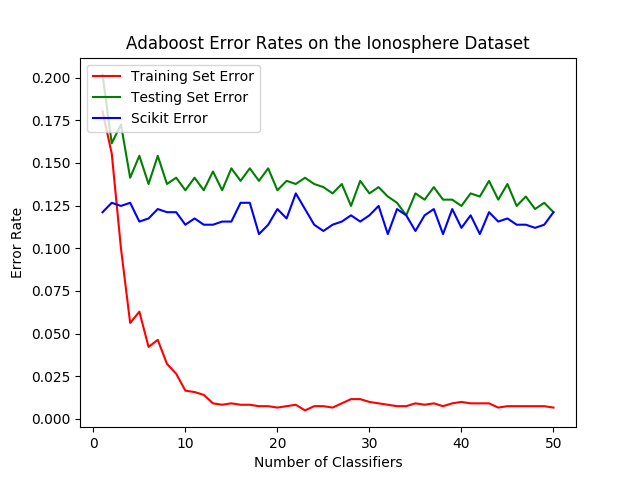
\includegraphics[scale=0.7]{Ionosphere_1}
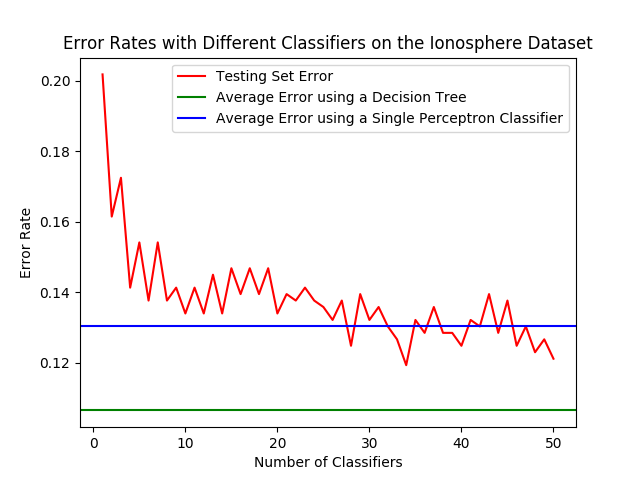
\includegraphics[scale=0.7]{Ionosphere_different_classifiers_1} 
\caption{The error rate on the testing and training sets drop dramatically with the first 10 classifiers. Adaboost does slightly better than a single perceptron classifier and consistently worse than a decision tree.}
\end{figure}

\begin{figure}[hbt]
\centering
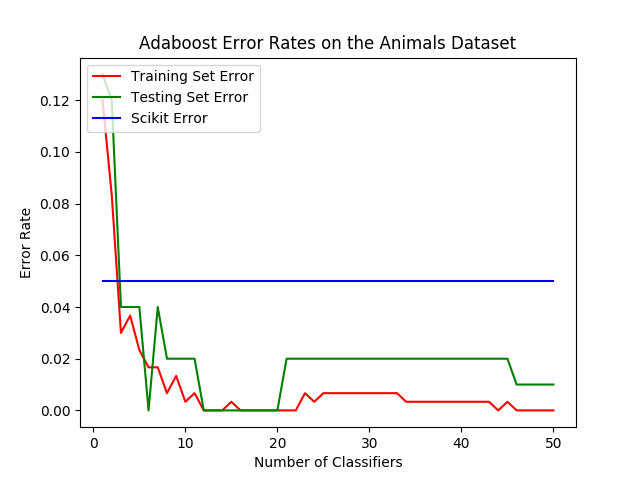
\includegraphics[scale=0.7]{Animals_1}
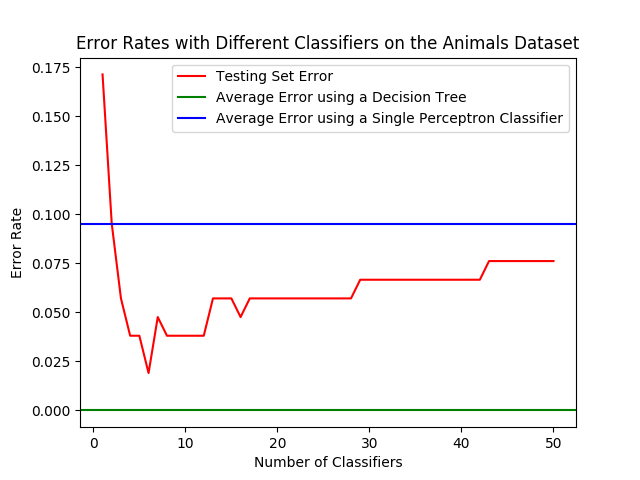
\includegraphics[scale=0.7]{Animals_different_classifiers_1} 
\caption{}
\end{figure}

\begin{figure}[hbt]
\centering
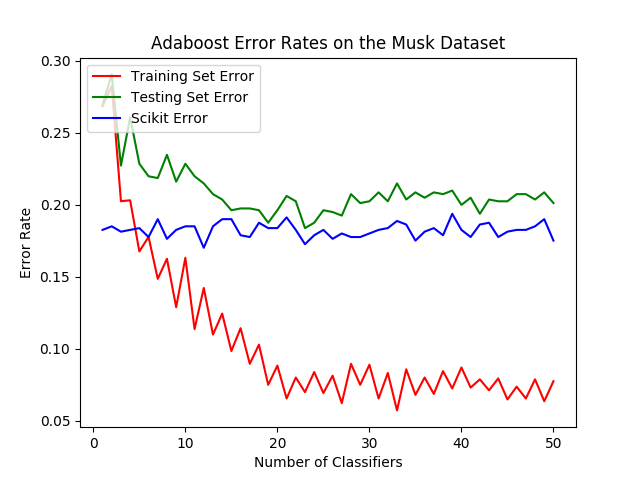
\includegraphics[scale=0.7]{Musk_1}
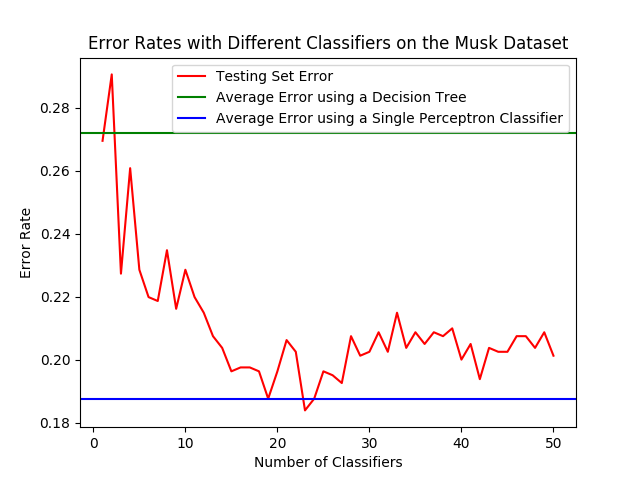
\includegraphics[scale=0.7]{Musk_different_classifiers_1} 
\caption{}
\end{figure}

\begin{figure}[hbt]
\centering
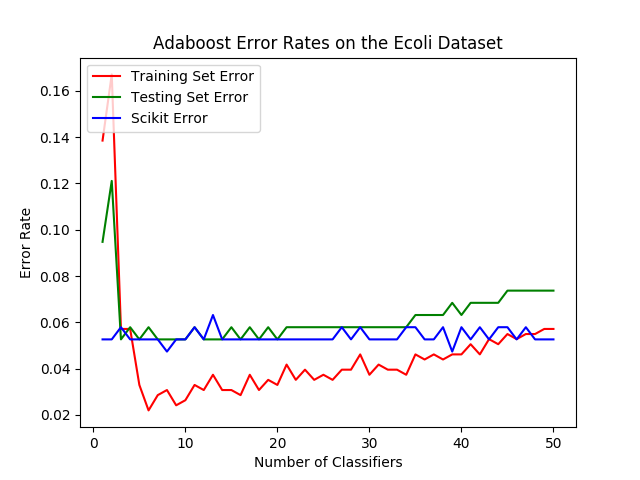
\includegraphics[scale=0.7]{Ecoli_1}
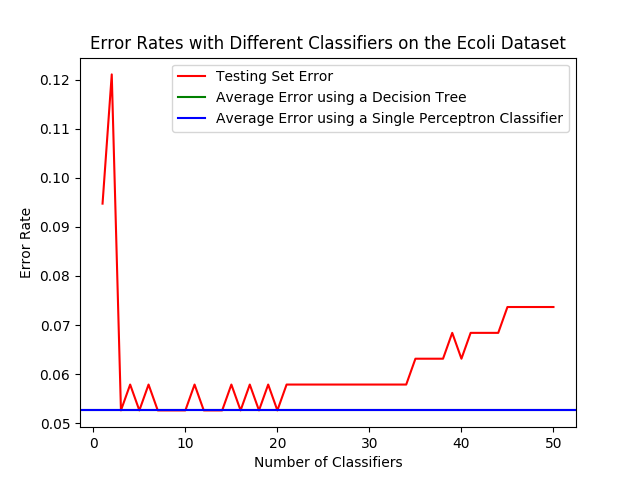
\includegraphics[scale=0.7]{Ecoli_different_classifiers_1} 
\caption{}
\end{figure}

\end{document}